\documentclass[parskip=full,11pt]{scrartcl}
\usepackage[utf8]{inputenc}
\usepackage[T1]{fontenc}
\usepackage[german]{babel}
\usepackage[useregional]{datetime2}
\usepackage[pdfborderstyle={/S/U/W 0}]{hyperref}
\usepackage[nameinlink]{cleveref}
\usepackage[section]{placeins}
\usepackage{xcolor}
\usepackage{graphicx}
\usepackage{csquotes}
\usepackage{amsmath} % for $\text{}$
\usepackage{pflichtenheft}

\newcommand\urlpart[2]{$\underbrace{\text{\texttt{#1}}}{\text{#2}}$}

\crefname{figure}{Abb}{Abb}

\hypersetup{
	pdftitle={Pflichtenheft},
	bookmarks=true,
}

% section numbers in margins:
\renewcommand\sectionlinesformat[4]{\makebox[0pt][r]{#3}#4}

% header & footer
\usepackage{scrlayer-scrpage}
\lofoot{\today}
\refoot{\today}
\pagestyle{scrheadings}

\newcommand\producttitle{GO-App}

\title{Pflichtenheft: \producttitle}
\author{Lukas Dippon
        \and Jens Kienle
        \and Matthias Noll
        \and Fabian Röpke
        \and Tim Schmidt
        \and Simon Vögele}

\begin{document}
\maketitle

\section{Einleitung}
Studenten und Mitarbeiter des KIT treffen sich gerne zum gemeinsamen Essen oder Lernen.
Dazu ist an einem bestimmten Tag immer notwendig zu wissen, ob bereits ein Treffen vereinbart wurde.
Am Treffpunkt angekommen, möchte man wissen, an welchem Ort sich die Gruppe befindet, um nicht lange suchen zu müssen.
Unsere App soll es angemeldeten Benutzern ermöglichen, sich in Gruppen zu organisieren.
In den Gruppen kann der Zeit- und Treffpunkt bestimmt werden.
Nach der Festlegung des Treffens soll die App die GPS-Standorte der Mitglieder temporär und anonym anzeigen, um das Treffen zu vereinfachen.

\pagebreak
\section{Kriterien}
% Diese Section sollte kurz und knapp "für Manager" sein
% und auf eine Seite passen.

\subsection{Muss}
\criterium{Vereinfachte Treffpunkte}{crt:easy}{10}
Durch das Freigeben von Positionsdaten können andere Nutzer den
Standort bestimmen.

\criterium{Datenschutz}{crt:safe}{20}
Die Positionsdaten werden nur mit Bestätigung
des Nutzers gesendet und serverseitig nicht längerfristig gespeichert.

\criterium{Gruppen}{crt:groups}{30}
Mehrere Nutzer können sich in Gruppen zusammenschließen. In diesen
können sie Positionsdaten austauschen und Treffpunkte festlegen.
Ein Nutzer kann in beliebig vielen Gruppen Mitglied sein.

\criterium{1 zu 1 Verbindung}{crt:1to1}{40}
Die Position kann auf Wunsch auch mit nur mit einem anderen Nutzer geteilt werden

\criterium{Account}{crt:acc}{50}
Ein persönlicher Account ermöglicht es allen Nutzern,
Gruppenzugehörigkeiten und Datenschutzoptionen zu speichern.

\subsection{Kann}
\criteriumOptional{Abstimmungen}{crt:vote}{10}
Innerhalb von Gruppen können die Nutzer z.B. über nächste Treffpunkte abstimmen

\criteriumOptional{Detailliertere Innenraumkarten}{crt:indoor}{20}
Innenräume mit hoher Nutzerdichte bekommen detaillierte Innenraumkarten.

\criteriumOptional{Seite mit Betreiberinfo}{crt:about}{30}
Der Dienst bietet eine Seite \enquote{Über Uns},
mit Informationen zum Betreiber.

\subsection{Abgrenzung}
\criteriumNot{Kein Social Network}{crt:socialNetwork}{10}
Die App bietet keine Plattform um Bilder oder andere persönliche Eindrücke mit Anderen zu teilen.

\criteriumNot{Kontakt nur zu Freunden}{crt:friendsOnly}{10}
Die App möchte die Kommunikation in bereits bestehenden Gruppen vereinfachen, nicht den Kontakt zu Fremden ermöglichen.

\criteriumNot{Nicht global}{crt:}{10}
Die Anwendung fokussiert sich auf das Gebiet rund um den Campus Süd des KIT.
Außerhalb dessen können manche Funktionen nur begrenzt zur Verfügung stehen.

\criteriumNot{Beidseitiges Einverständnis}{crt:}{10}
Die Anwendung ermöglicht nicht das Positionieren von Personen, die ihre Position nicht ausdrücklich
zugänglich machen. Beispielsweise können insbesondere Eltern nicht ihre Kinder ständig mit dieser App orten.

\pagebreak
%%%%%%%%%%%%%%
\section{Produkteinsatz}
Das Produkt dient zur Erleichterung des Zusammenfindens und der
Treffpunktvereinbarung in geschlossenen Gruppen von Freunden, Kollegen oder
Familienmitgliedern.

\subsection{Anwendungsbereiche}
\begin{itemize}
    \item Private Treffen in der Freizeit oder während der Arbeit
    \item Zusammenfindung auf größeren Veranstaltungen
\end{itemize}

\subsection{Zielgruppen}
\begin{itemize}
    \item Freundesgruppen
    \item Arbeitskollegen
\end{itemize}

\subsection{Betriebsbedingungen}
\begin{itemize}
    % TODO: Unschön formuliert
    \item Mobiler Einsatz in Umgebungen mit GPS-Empfang
\end{itemize}

%%%%%%%%%%%%%%
\section{Produktumgebung}
Das Produkt beinhaltet ein Client-Server-Modell.
Der Server dient lediglich als Vermittler zwischen Klienten.
Die Nutzer verwenden den Klienten auf ihrem mobilen Endgerät.
\subsection{Software}
\begin{itemize}
    \item Client: Android 4.1 (\enquote{Jelly Bean}, API-Level 16) oder
        höher.
    \item Server: Apache Tomcat 8
\end{itemize}

\subsection{Hardware}
% TODO: Mindestanforderungen an Hardware-Performance
\begin{itemize}
    \item Client: Android-fähiges mobiles Endgerät mit
        \begin{itemize}
            \item GPS-Empfänger
            \item Netzwerkkarte mit WLAN-Modul oder Mobilfunkeinheit
        \end{itemize}
    \item Server: Beliebiger Servercomputer, der Apache Tomcat 8 unterstützt
        und eine Internetanbindung besitzt
\end{itemize}

%%%%%%%%%%%
\section{Funktionale Anforderungen}

\functionality{Homepage der App unterteilt in Tabs für die unterschiedlichen Funktionen}{fnc:ui}{10}
\begin{itemize}
    \item Liste aller Gruppen, in denen man Mitglied ist (\functionalitylink{fnc:groupfounding})
    \item Liste aller Events, an welchen man teilnimmt (\functionalitylink{fnc:events})
    \item Einstellungen(\functionalitylink{fnc:options})
\end{itemize}

\functionality{Login in einen appspezifischen Account}{fnc:login}{20}
\fulfills{crt:acc}
Der Benutzer muss sich vor der Nutzung der App einen Account erstellen und sich mit diesem einloggen.

\functionality{Verwaltung von Einstellungen und Account- oder appbezogene Daten}{fnc:options}{30}
\fulfills{crt:acc}
Platzhalter % TODO: Beschreibung

\functionality{Gründen von Gruppen}{fnc:groupfounding}{40}
\fulfills{crt:groups}
Über einen Reiter im Hauptmenü können Gruppen erstellt werden.
Ihre Funktionen werden in \functionalitylink{fnc:groupmenu} bis \functionalitylink{fnc:locations} beschrieben.

\functionality{Gruppenmenü}{fnc:groupmenu}{50}
\fulfills{crt:groups}
Jede Gruppe besitzt ein eigenes Menü über welches ihre Funktionen angesteuert werden können:
\begin{itemize}
    \item Umgebungskarte (\functionalitylink{fnc:map})
    \item Anfrage von GPS-Standorten (\functionalitylink{fnc:locationrequest})
    \item Erstellen eines Events (\functionalitylink{fnc:events} und \functionalitylink{fnc:vote})
    \item Einladen von Mitgliedern (\functionalitylink{fnc:invitations})
    \item Liste aller Mitglieder (\functionalitylink{fnc:memberlist})
\end{itemize}

\functionality{Einladen von Mitgliedern}{fnc:invitations}{60}
\fulfills{crt:groups}
Es können Einladungen an Nutzer versandt.
Diese können von den eingeladenen Nutzern akzeptiert oder abgelehnt werden.

\functionality{Liste der Gruppenmitglieder}{fnc:memberlist}{70}
\fulfills{crt:groups}
Es werden alle Mitglieder aufgelistet.
Durch das Anklicken eines Mitgliedes kann wahlweise das zugehörige Profil besucht oder das Mitglied aus der Gruppe entfernt werden.

\functionality{Umgebungskarte}{fnc:map}{80}
\fulfills{crt:groups}
\fulfills{crt:easy}
Jede Gruppe verfügt über eine Umgebungskarte mit eigenem Standort.

\functionality{Anfrage von GPS-Standorten}{fnc:locationrequest}{90}
\fulfills{crt:groups}
\fulfills{crt:easy}
Erstellen einer GPS-Anfrage, bei der alle Gruppenmitglieder über ein Pop-Up gebeten werden ihren Standort für einen fest definierten Zeitraum freizugeben

\functionality{Anzeigen von anonymen GPS-Standorten}{fnc:locations}{100}
\fulfills{crt:easy}
\fulfills{crt:safe}
Alle GPS-Standorte der Grupenmitglieder, die aktuell freigestellt sind, werden erfasst und als Gruppierungen auf der in \functionalitylink{fnc:map} beschriebenen Gruppenkarte markiert.
Diese Gruppierungen bestehen aus geographisch nah beieinanderliegenden Gruppenmitgliedern.
Einzelpersonen werden dabei unterscheidbar von Gruppierungen symbolisiert.

\functionality{Events}{fnc:events}{110}
Gruppenmitglieder können ein Event, bestehend aus Ort und einen Zeit, definieren.
Das Event wird mit Uhrzeit in der Eventliste(\functionalitylink{fnc:eventlist}) aufgelistet und mit Uhrzeit auf der Karte (\functionalitylink{fnc:map}) markiert.
Die Mitglieder werden eine kurze Zeit vor dem Event automatisch von der App über ein Pop-Up gebeten, ihren Standort temporär freizugeben.

\functionality{Abstimmungen}{fnc:vote}{120}
\fulfills{crt:vote}
Das Event(\functionalitylink{fnc:events}) lässt sich durch eine Abstimmung vereinbaren.
Diese ist zeitlich begrenzt durch eine vom Ersteller festgelegte Zeit.
Hierbei können inerhalb der Zeitgrenze beliebig oft von den Gruppenmitgliedern Orte und Zeitpunkte hinzugefügt werden, die eigene Stimme verändert, oder die Zeitgrenze verlängert werden.

\functionality{Anzeigen von Treffpunkten}{fnc:meetingpoints}{130}
\fulfills{crt:vote}
\fulfills{crt:easy}
Während einer Abstimmung werden alle möglichen Orte auf der Karte (\functionalitylink{fnc:map}) als solche angezeigt.
Durch das Anklicken des Ortes in der Abstimmung lassen sich die Markierungen auf der Karte erreichen.
Nach Vollendung der Abstimmung wird der Ort mit den meisten Stimmen als finaler Treffpunkt festgelegt, während alle anderen Orte von der Karte gelöscht werden.

\functionality{Standortteilung für einzelne Personen}{fnc:1to1}{140}
\fulfills{crt:1to1}
\fulfills{crt:easy}
Es soll auch für Einzelpersonen möglich sein ihren Standort zu teilen.
Dies soll intern als Zweiergruppe implementiert sein, aber in der App als extra Reiter schnell und ohne den Umweg über die Gruppengründung möglich sein.

\functionality{Eventliste}{fnc:eventlist}{150}
Alle vereinbarten Treffen werden nach Zeitpunkt sortiert angezeigt.
Das Auswählen eines Treffens zeigt die aktuelle Umgebungskarte(\functionalitylink{fnc:map}) der entsprechenden Gruppe an.

%%%%%%%%%%%
\section{Nicht-Funktionale Anforderungen}

\nonFunctionality{Modernes Design}{nfc:design}{10}

Das Design soll modern und seriös wirken.

\nonFunctionality{Persistenz}{nfc:persistence}{20}

Sollten in Zukunft Erweiterungen oder Updates notwendig werden,
müssen die Daten (Kurz-URLs, E-Mailaddressen) erhalten bleiben.

\nonFunctionality{Erweiterbarkeit}{nfc:extensibility}{30}

Das Produkt muss dahingehend erweiterbar sein,
das die Liste der E-Mail-URL Abbildung von authentifizierten Nutzern
abgerufen werden kann.
Wie das genau implementiert wird, ist nicht Teil dieses Projekts.

%%%%%%%%%%%
\section{Tests}

\test{Gruppe Erstellen}{tst:grpcreate}{10}
\tests{fnc:login}

\teststep{Nutzer \enquote{Ned Stark} ist eingeloggt.}
{Ned tippt auf den Tab  \enquote{Gruppen}.}
{Er bekommt die Liste aller Gruppen angezeigt in denen er Mitglied ist.}

\teststep{Ned möchte eine Gruppe mit Leuten aus dem Fußball-Training erstellen.}
{Er tippt auf den \enquote{+}-Button (Neue Gruppe erstellen).}
{Er bekommt eine Liste all seiner Kontakte, die er im Produkt hinzugefügt hat, angezeigt.}

\teststep{Seine Freunde Robert B. und Edmund T. spielen ebenfalls Fußball.}
{Er tippt die beiden Namen an.}
{Das Produkt schlägt ihm vor die Gruppe zu erstellen.}

\teststep{Ned hat keine weiteren Freunde.}
{Er tippt auf Gruppe erstellen}
{Der Homescreen der Gruppe wird angezeigt.} % TODO: Homescreen?

%%%%%%%%%%%%%
\pagebreak
\appendix

\section{Seitenentwürfe}

% made via https://gomockingbird.com/projects/mnf0cwf/4gXVnC

\begin{figure}[hb]
	\fbox{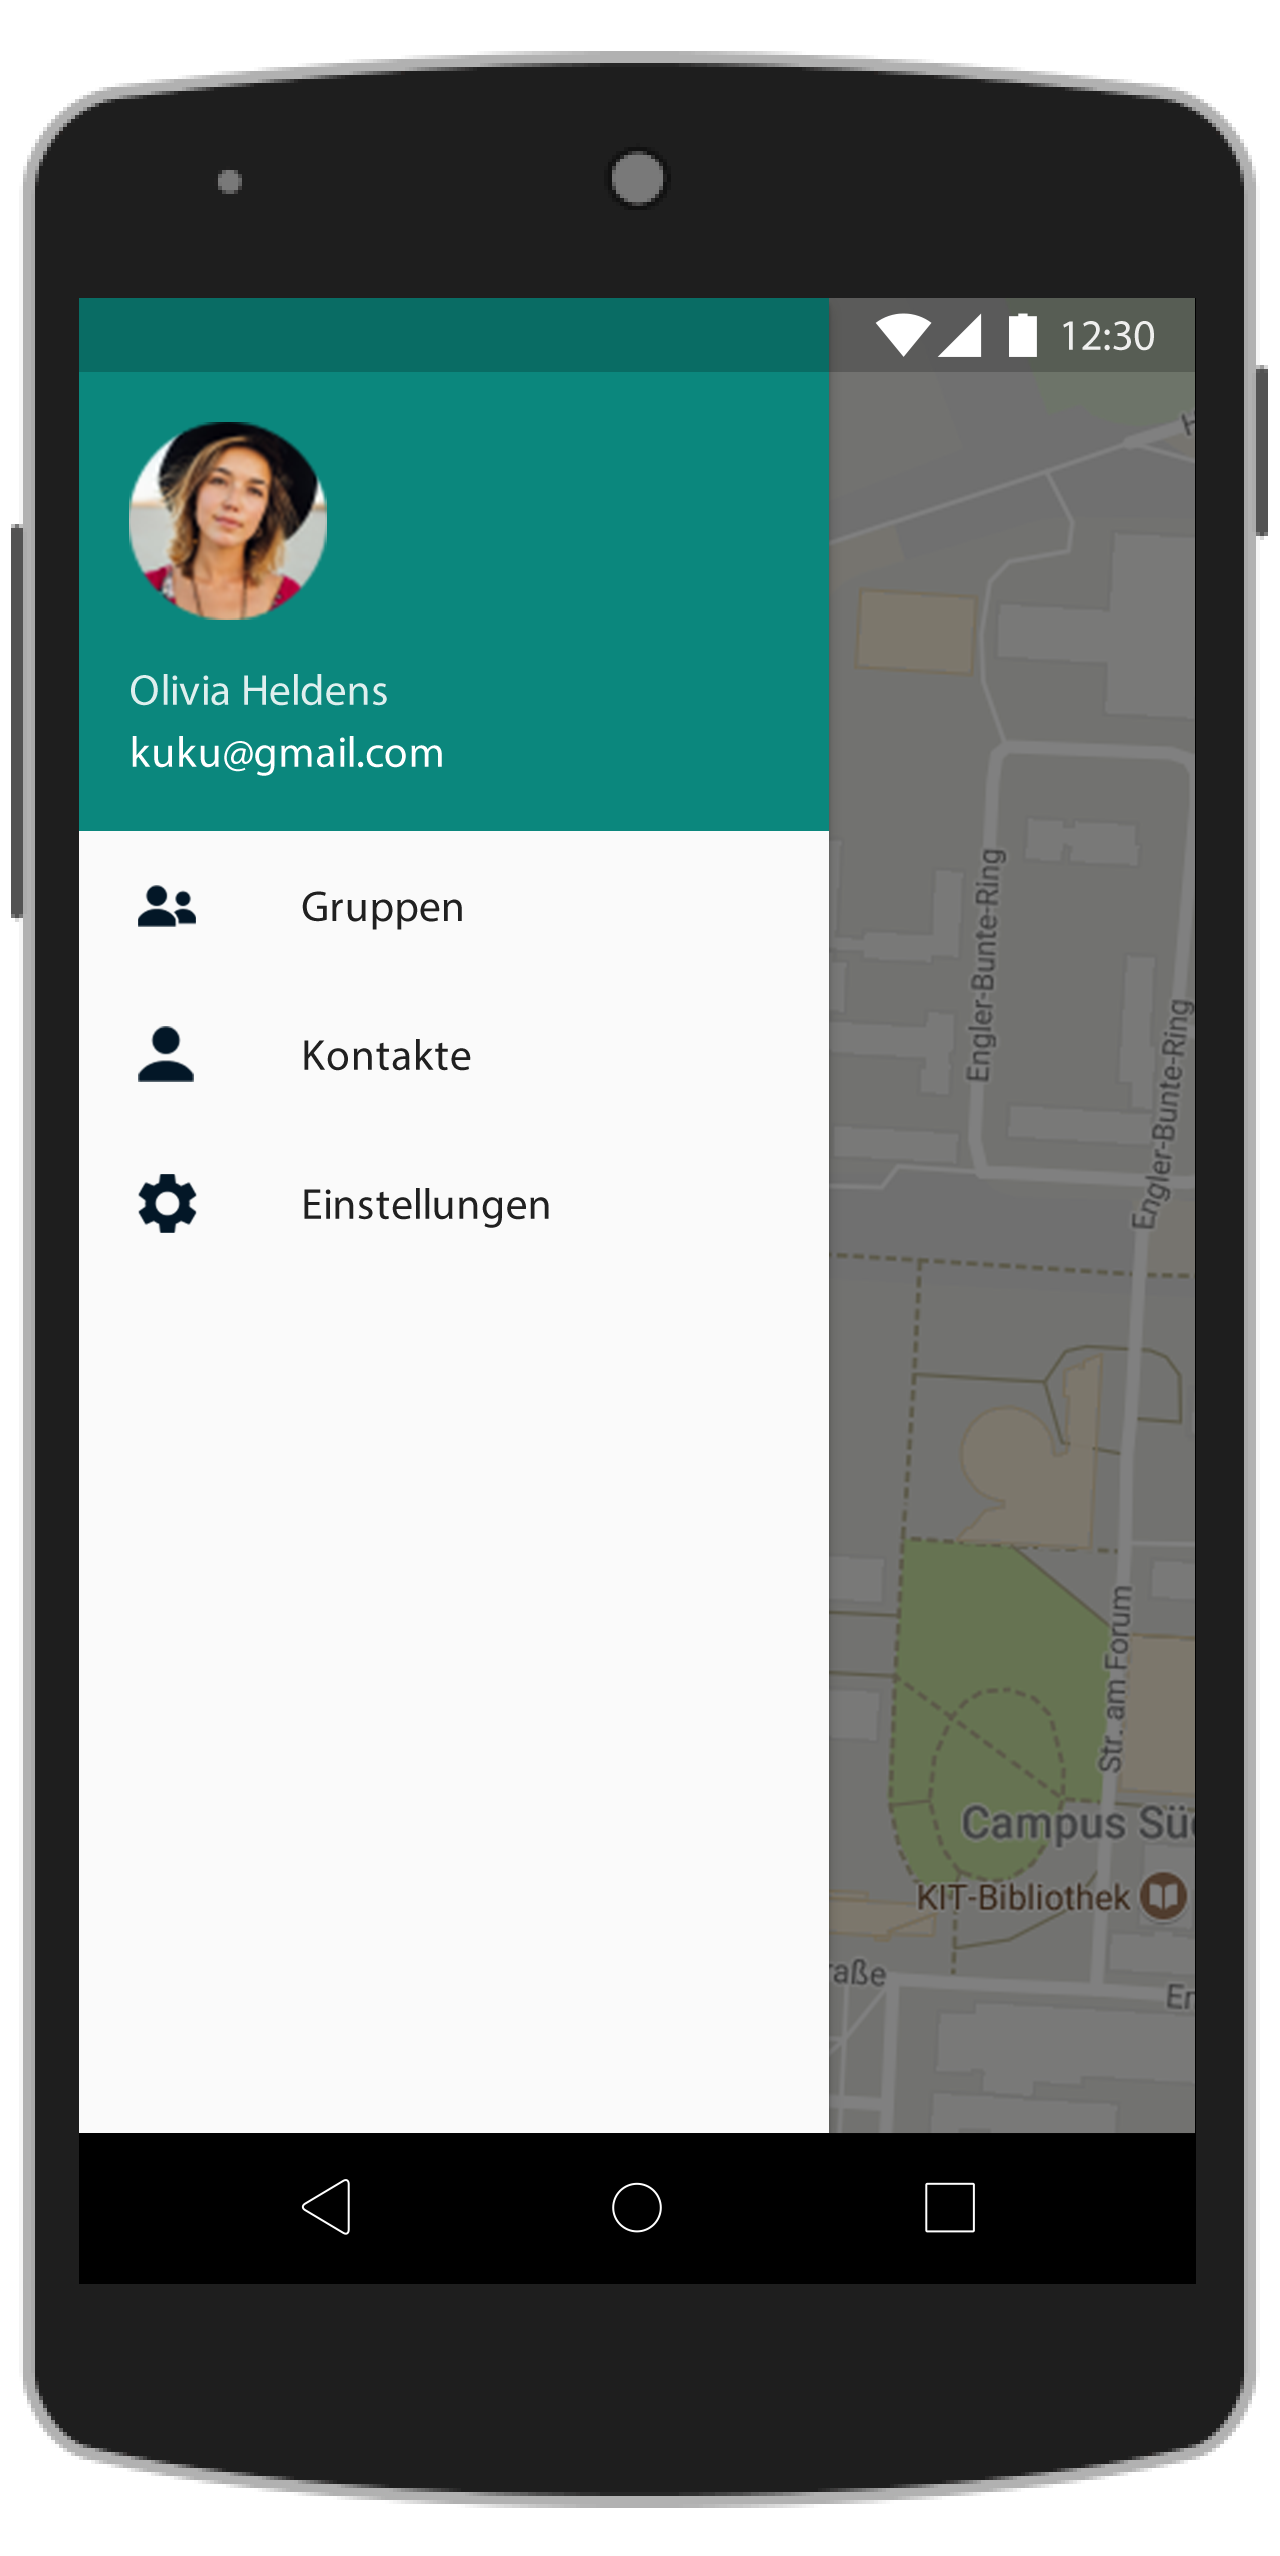
\includegraphics[height=80mm]{screenshots/menu.png}}
	\caption{\label{fig:menu}
		Menü mit der Möglichkeit auf Gruppen, Kontakte und Einstellungen zuzugreifen.
		 \testlink{tst:grpcreate}.
	}
\end{figure}

\begin{figure}[hb]
		\fbox{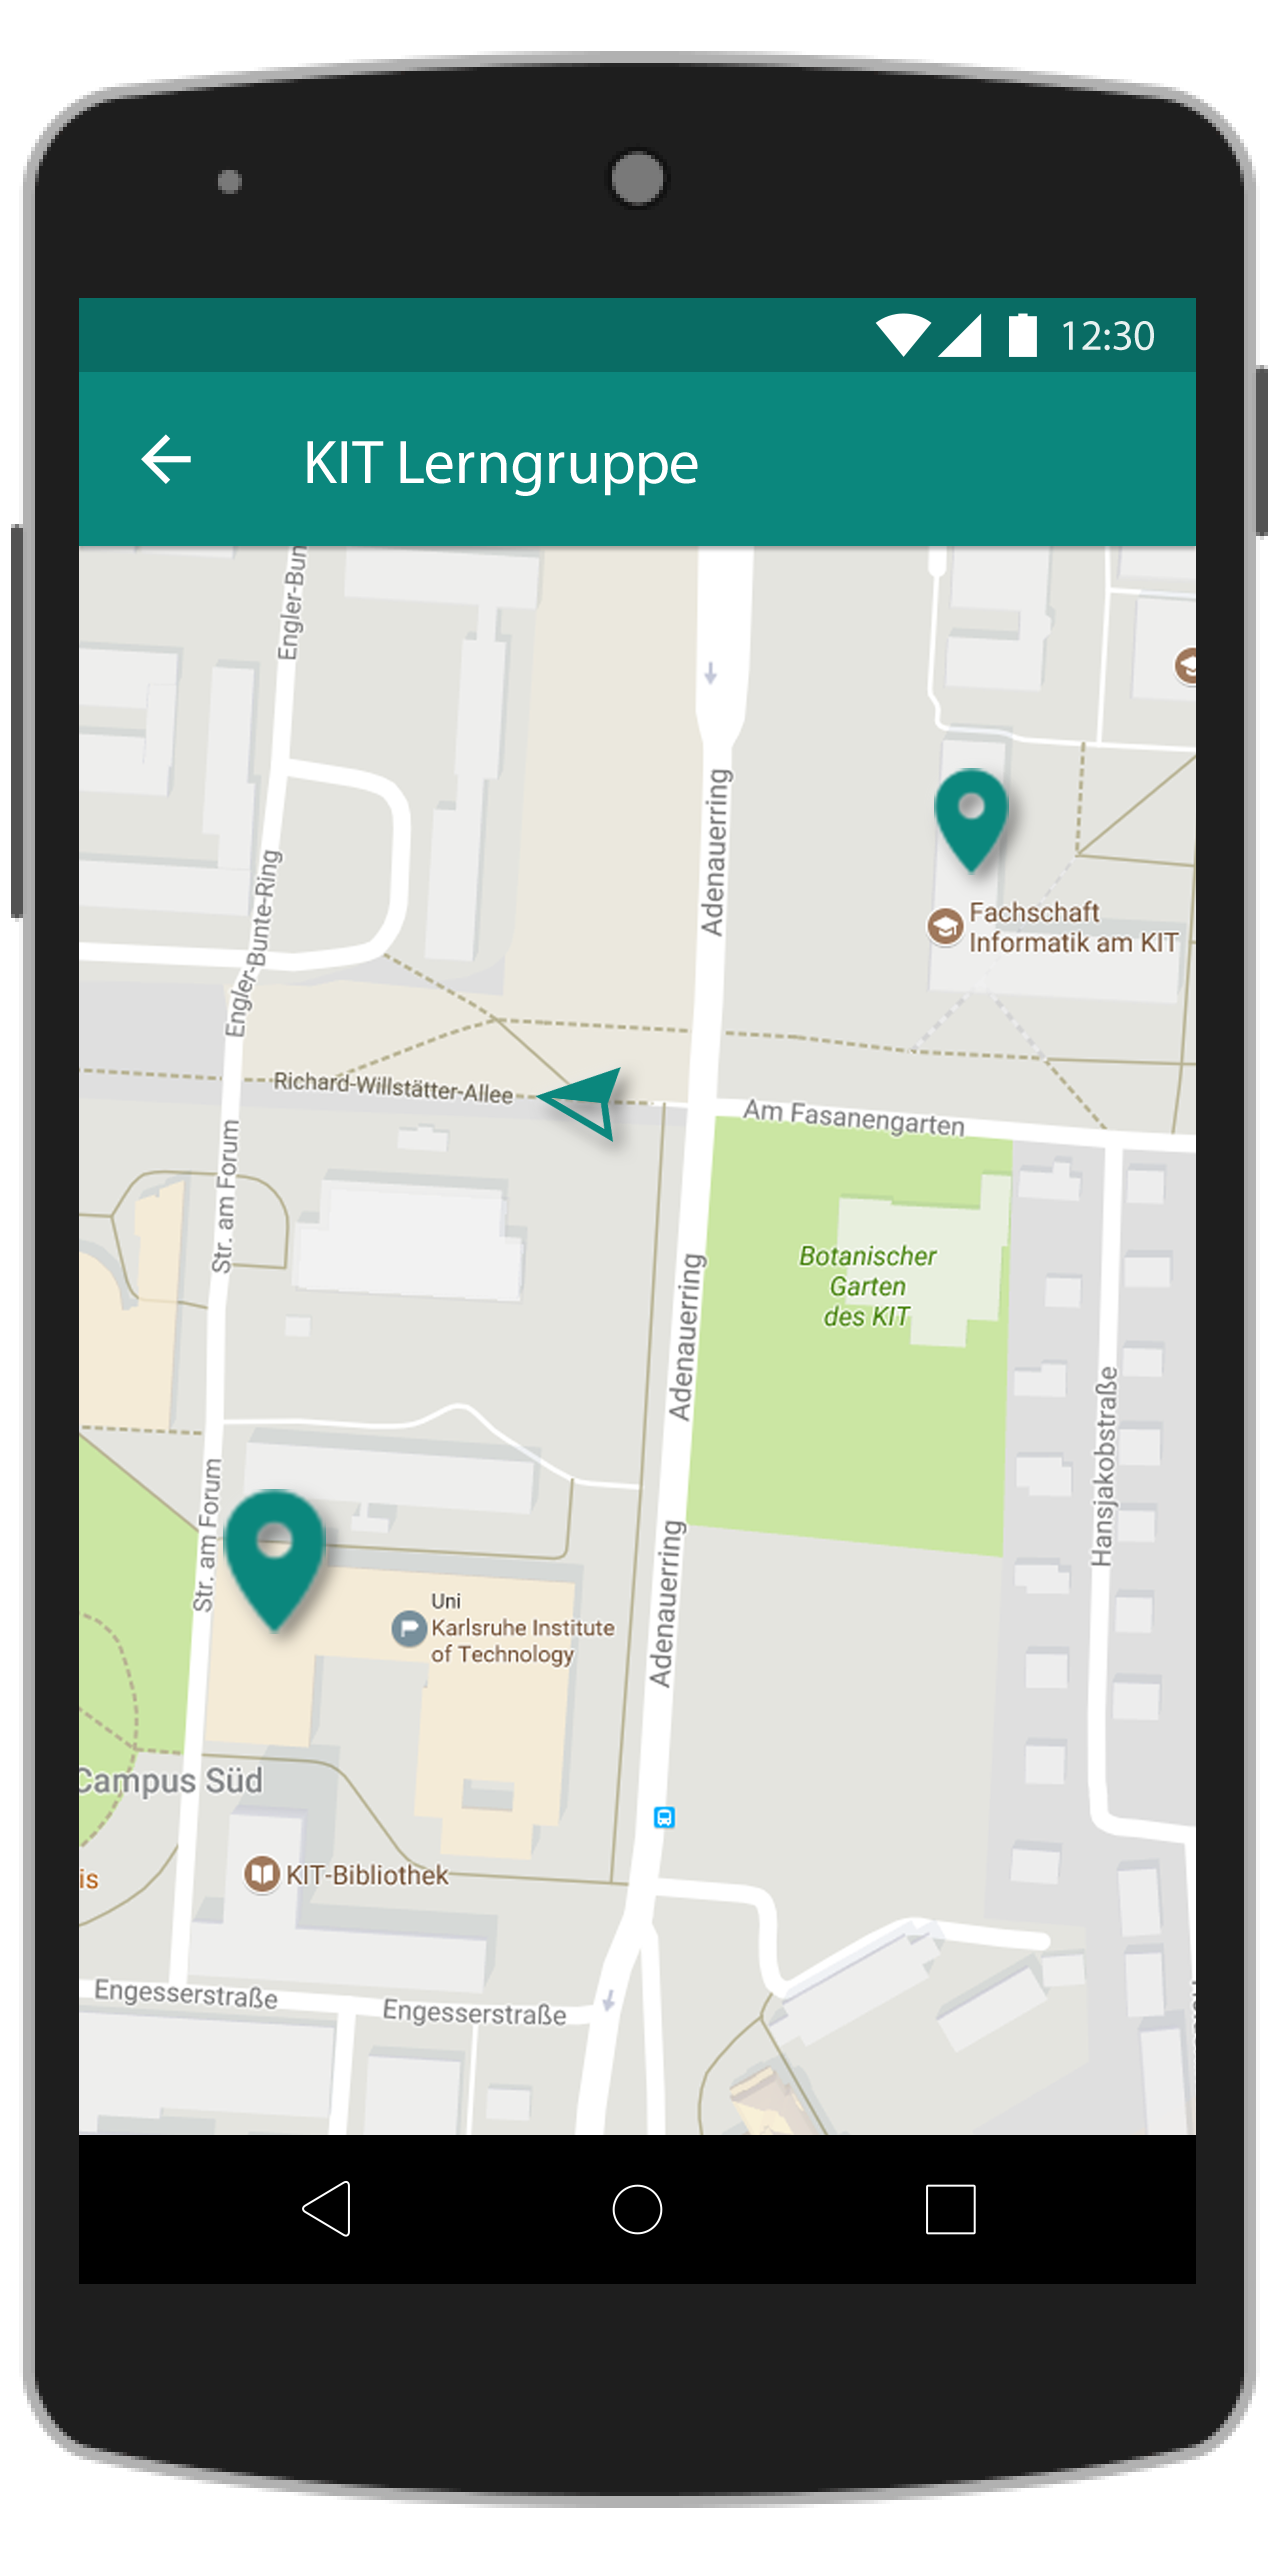
\includegraphics[height=80mm]{screenshots/karte.png}}
		\caption{\label{fig:map}
			Auf der Karte kann die Position der anderen Gruppenmitglieder eingesehen werden.
			Orte mit mehreren Mitgliedern erscheinen größer.
			\testlink{tst:grpcreate}.
		}
\end{figure}

\begin{figure}[hb]
		\fbox{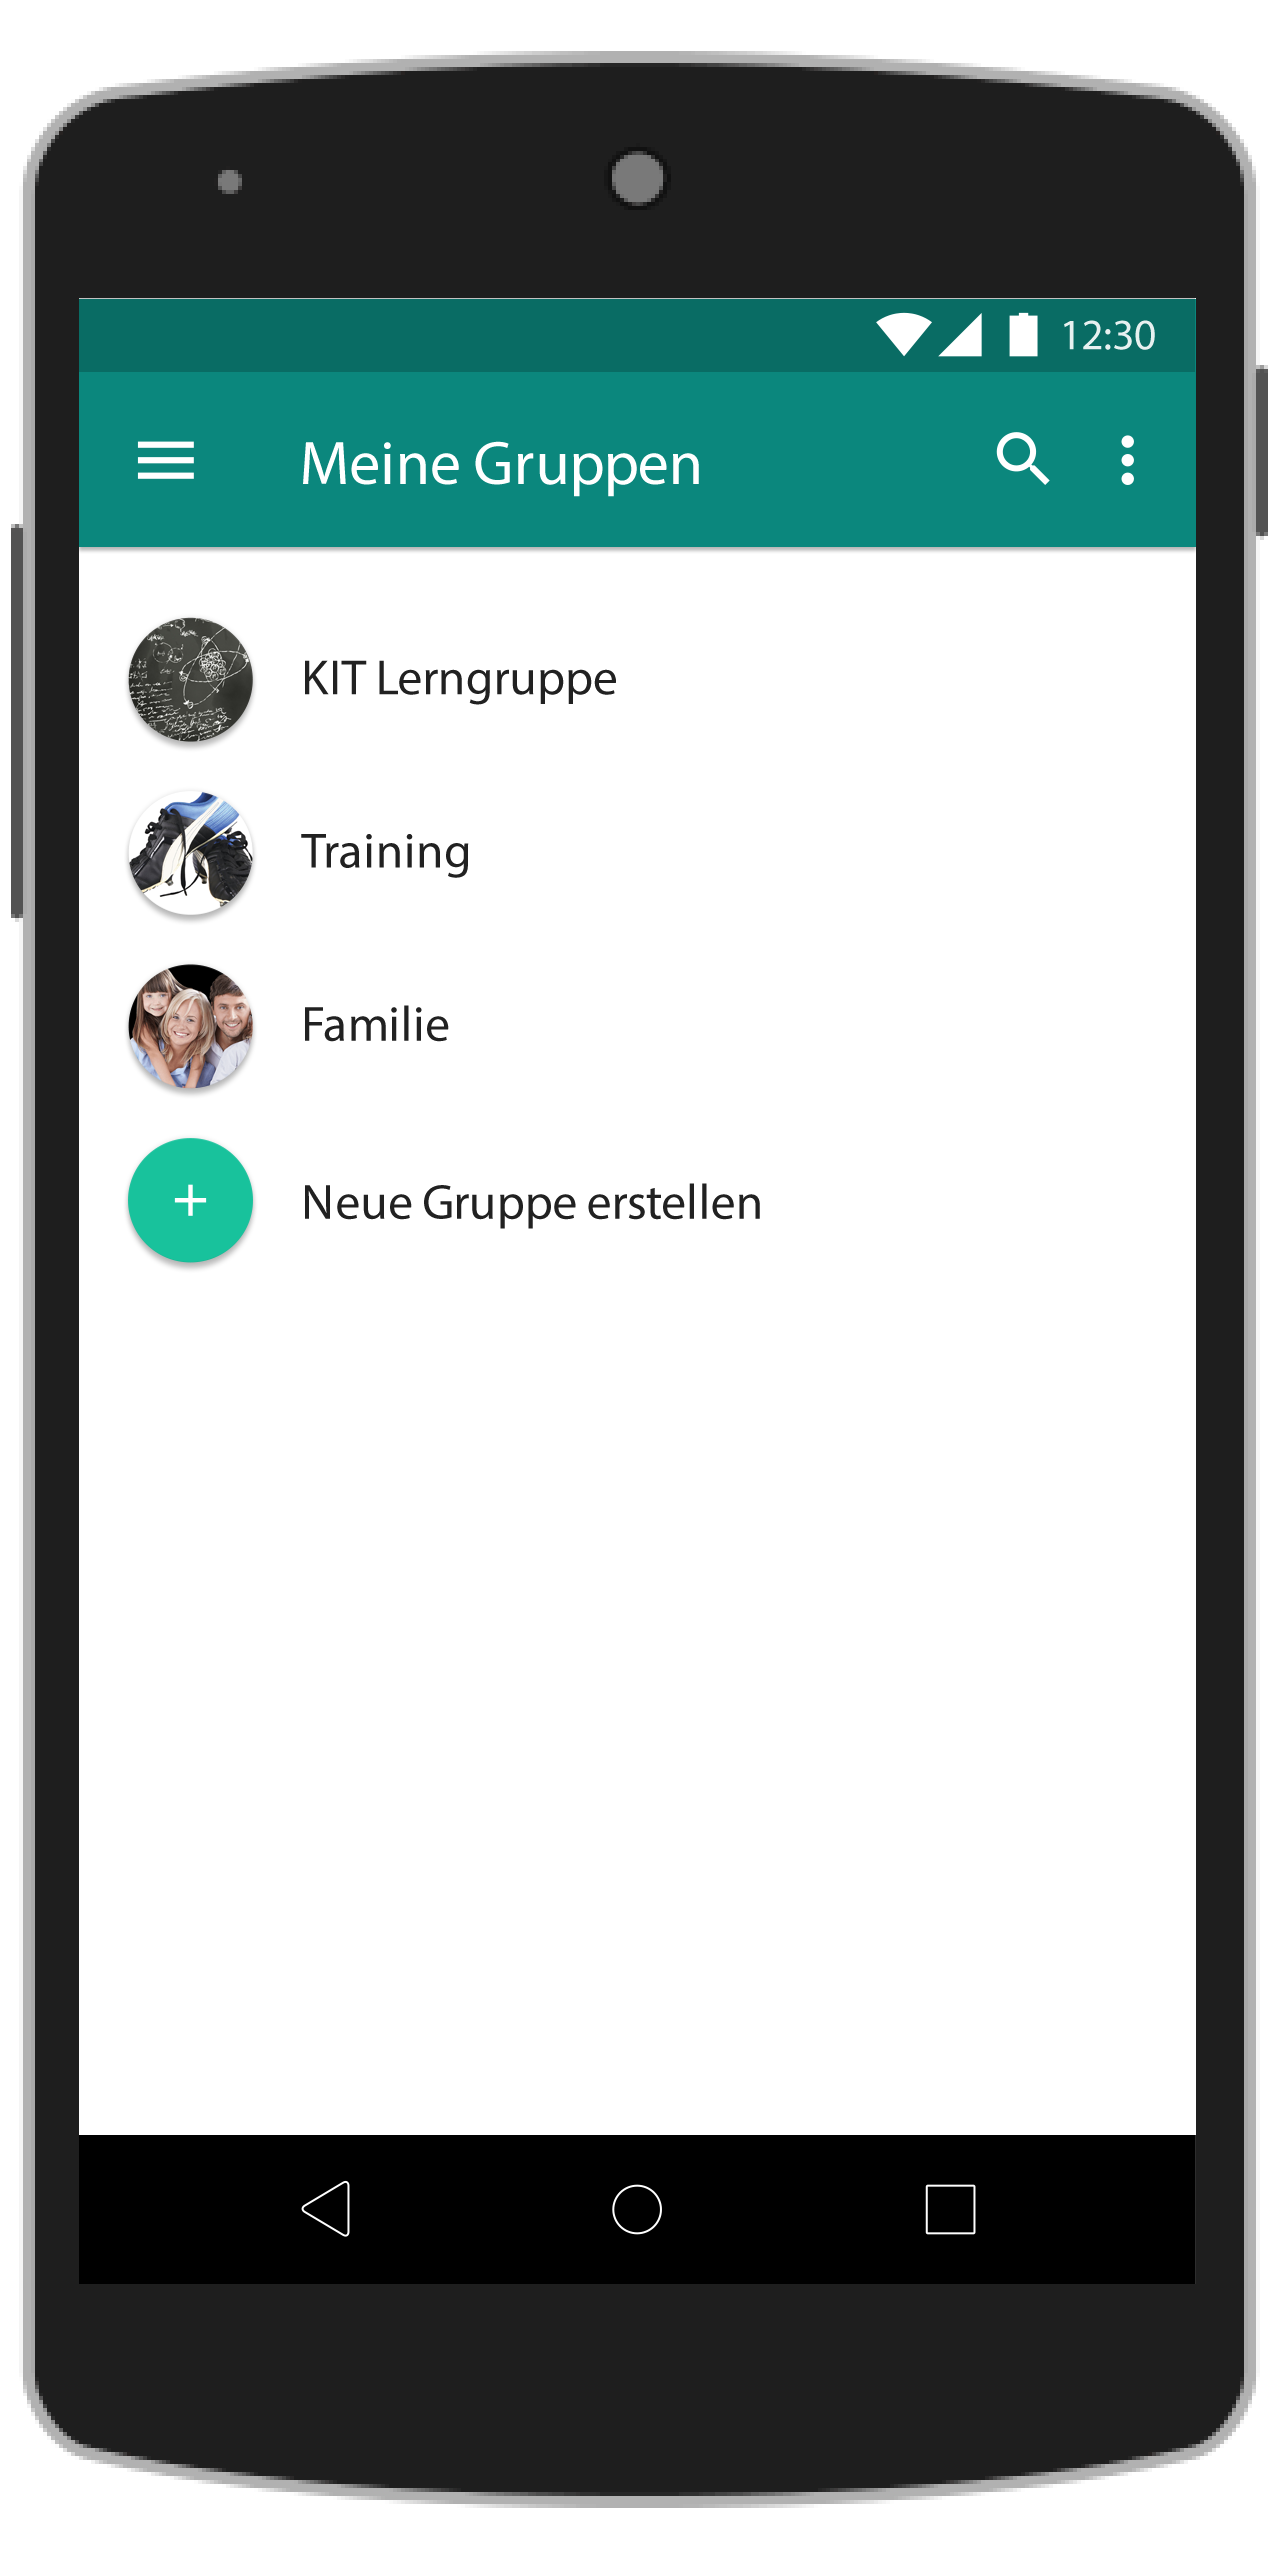
\includegraphics[height=80mm]{screenshots/gruppen.png}}
		\caption{\label{fig:groups}
			Hier können Gruppen verwaltet und angesehen, sowie neue hinzugefügt werden.
			\testlink{tst:grpcreate}.
		}
\end{figure}

\section{Glossar}

\textbf{Besucher}:
Eine Person, welche den Dienst nutzt.
Kann eingeloggt sein oder nicht.

\textbf{Dienst}:
Die Software im laufenden Betrieb. Software as a Service.

\textbf{Homepage}:
Seite, die beim Besuchen der Betreiberdomain \emph{ohne Pfad} angezeigt wird. Auch \enquote{Startseite}.

\textbf{Nutzer}:
Ein eingeloggter Besucher.

\end{document}
